\documentclass{article}
\usepackage{graphicx} % Required for inserting images
\usepackage[left=1.5cm, right=1.5cm, top=1.5cm]{geometry}
\usepackage{enumitem}
\usepackage{amsmath}
\usepackage{amsfonts}
\usepackage{listings}
\usepackage{xcolor}

\usepackage[utf8]{inputenc}
\definecolor{dkgreen}{rgb}{0,0.6,0}
\definecolor{mauve}{rgb}{0.58,0,0.82}

\lstset{frame=tb,
  language=Bash,
  aboveskip=3mm,
  belowskip=3mm,
  showstringspaces=false,
  columns=flexible,
  basicstyle={\small\ttfamily},
  numbers=none,
  numberstyle=\tiny\color{gray},
  keywordstyle=\color{blue},
  commentstyle=\color{dkgreen},
  stringstyle=\color{mauve},
  breaklines=true,
  breakatwhitespace=true,
  tabsize=4
}
\title{Distributed Systems: Assignment 3a}
\author{Deven Mistry}
\date{March 13th, 2025}
\setlength\parindent{0pt}
\begin{document}

\maketitle

\section{Introduction}

In this asssigment, we setup four `Stateful' pods in Kubernetes for our container. The entire idea in the third assignment is to have ring communication in the network, where when a message is sent from the first node, it is relayed to the second node and third and so on. For now, in my submission, I have created the containers in my local Kubernetes.

\section{Building containers}

I personally struggled the most in this part of the assignment. I was unable to build the docker container, as I thought there was a typo in the instructions, where after cloning the repository, we change the directory to the `container' directory.

However, to build the container, once the repository was cloned initally, after changing the directory to `container', we were supposed to clone the repository again inside the `container' directory. Following the instructions then, made the process of building containers extremely straightforward. Here are the steps that I had followed.

\begin{lstlisting}
    git clone git@github.iu.edu:swany/dist-sys
    eval $(minikube docker-env)

    cd container

    # this is not a typo, we clone the repo again
    # inside the container folder
    git clone git@github.iu.edu:swany/dist-sys
    docker build -t=dms .
\end{lstlisting}

Once the container was built, runnning
\begin{lstlisting}
    docker image ls
\end{lstlisting}

showed the built image.

\begin{center}
    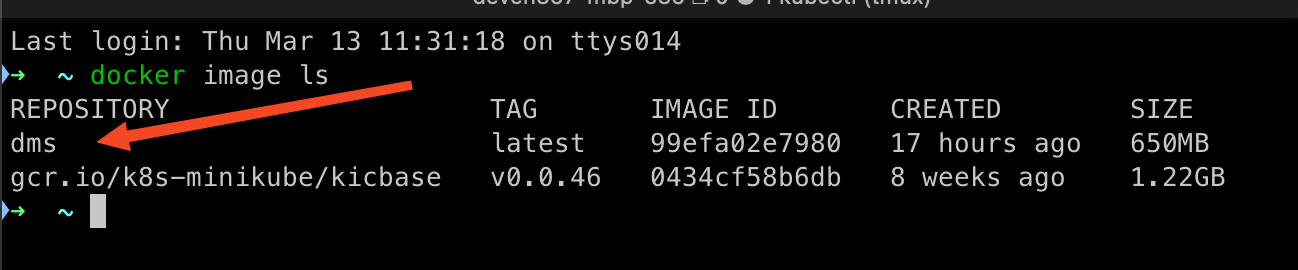
\includegraphics[scale=0.5]{docker-img.png}
\end{center}

\section{Running containers}

After building the container, creating and running the pods is straightforward. We create the pods the given yaml files and run the pods.

\begin{lstlisting}
    kubectl apply -f dms-service.yaml
    kubectl apply -f dms-sset.yaml
\end{lstlisting}

We verify the pods, were created using

\begin{lstlisting}
    kubectl get pods
\end{lstlisting}

\begin{center}
    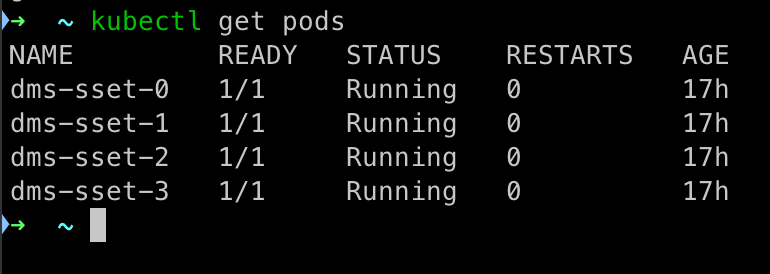
\includegraphics[scale=0.5]{pods.png}
\end{center}

We now login and start the service and open a shell in each node.

I use a `tmux' session for this step

\begin{lstlisting}
    kubectl exec --stdin --tty dms-sset-0 -- /bin/bash
    kubectl exec --stdin --tty dms-sset-1 -- /bin/bash
    kubectl exec --stdin --tty dms-sset-2 -- /bin/bash
    kubectl exec --stdin --tty dms-sset-3 -- /bin/bash
\end{lstlisting}

To have the client communicate with the server, we need the server's IP address, which we obtain through

\begin{lstlisting}
    ifconfig eth0
\end{lstlisting}

Once we have the IP address, we start the server on the first node (node-0) and listen to port 2525 (as specified in the yaml config), and on node-1, we start the client. To chat with the server, we give it the IP address and port of the server obtained from the output of the previous command.

\begin{lstlisting}
    # to start server on node-0
    /bin/dserver -l 2525

    # to start client on node-1
    /bin/dclient -c 10.244.0.4:2525

\end{lstlisting}

The server is expecting a tuple separated by comma, we send a message and see the server receive it.

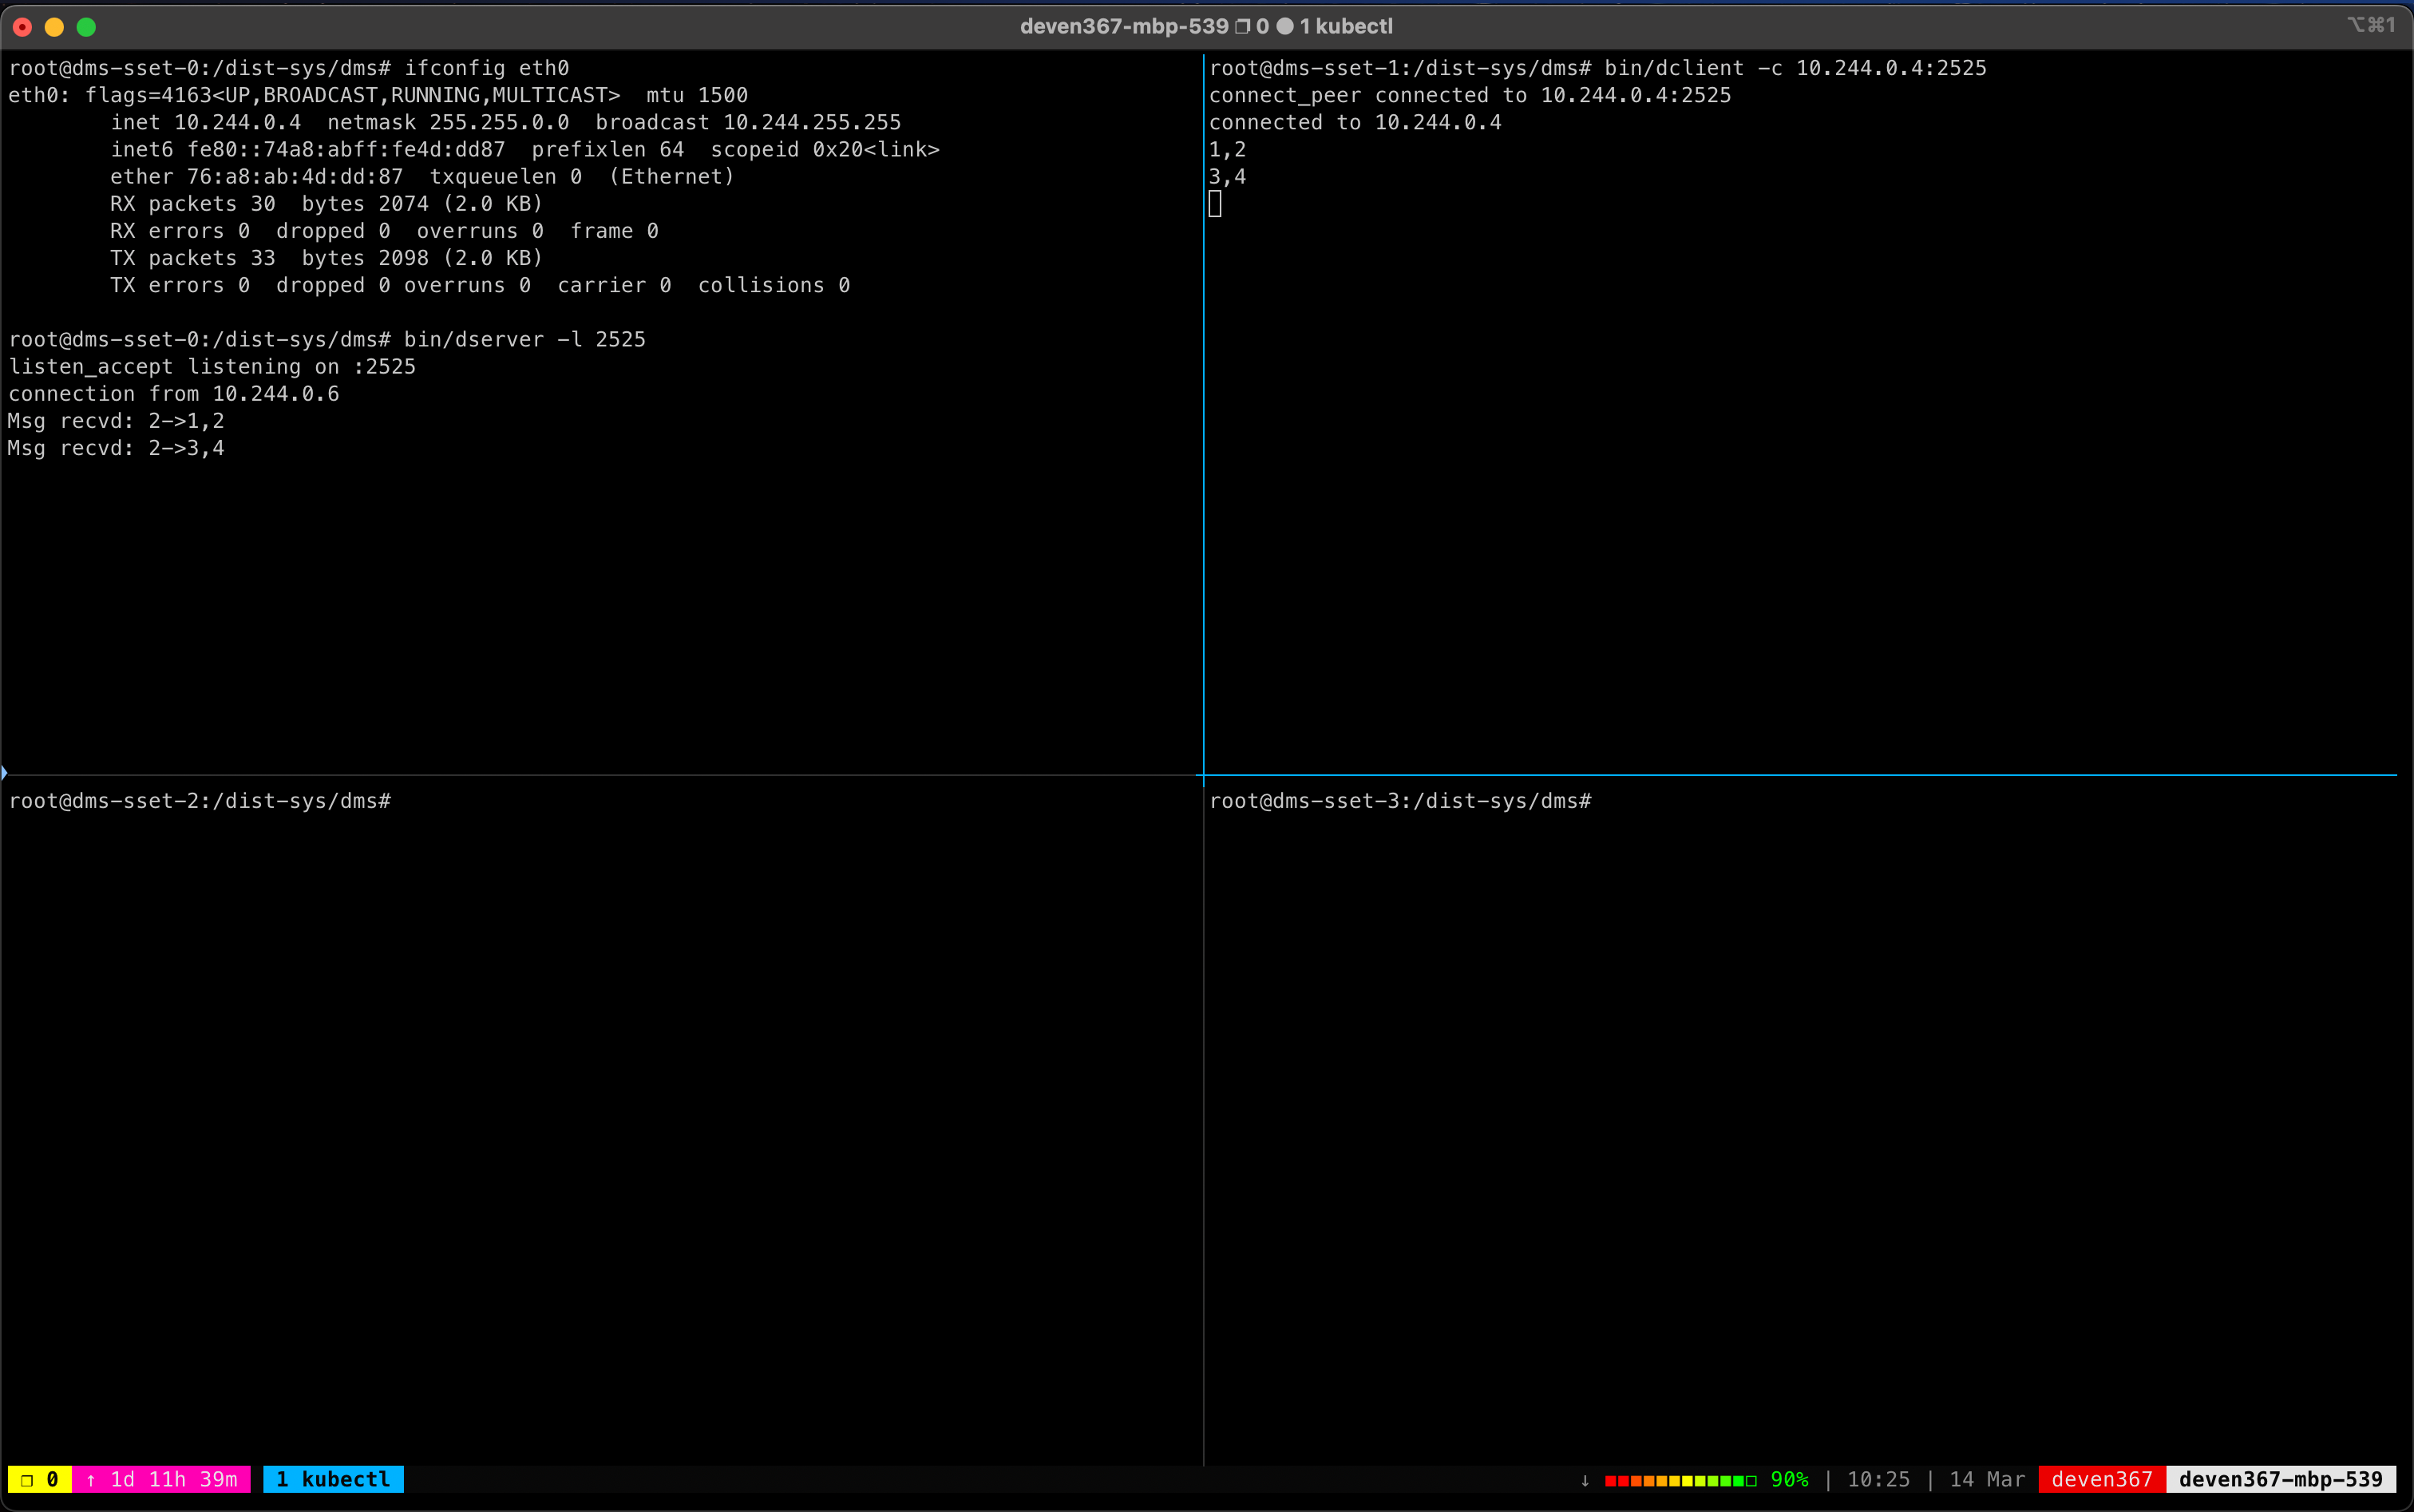
\includegraphics[scale=0.345]{final-output.png}

\end{document}